%%%%%%%%%%%%%%%%%%%%%%%%%%%%%%%%%%%%%%%%%
%
% Funkcionalna verifikacija hardvera
% 
%%%%%%%%%%%%%%%%%%%%%%%%%%%%%%%%%%%%%%%%%

Osma vežba je posvećena monitoru. Detaljnije su objašnjene TLM konekcije, dat je
opis strukutre i funkcionalnosti UVM monitora i objašnjen preporučen način
pisanja čekera.

%========================================================================================
% Section
%========================================================================================

\section{TLM}

Prilikom razvoja verifikacionog okruženja potrebno je problemu pristupiti na
odgovarajućem nivou apstrakcije. Iako je interfejs ka DUT-u reprezentovan na
nivou signala, u praksi se pokazalo da je za većinu taskova u verifikaciji
(generisanje stimulusa, analiza podataka, prikupljanje pokrivenosti, ...)
efikasnije posmatrati problem na nivou transakcija. UVM pruža velik skup
interfejsa za komunikaciju na nivou transakcija. Korišćenje ovih TLM
(\emph{Transaction Level Modeling}) interfejsa omogućava izolaciju komponenti
tako da promene u okruženju ne utiču na datu komponentu. Ovim postupkom se
omogućava laka ponovna upotreba, ali i jednostavna zamena komponenti do god
sadrže isti interfejs.\\

TLM-1 i TLM-2.0 su dva TLM sistema modelovanja implementirana po industrijskim
standardima. Oba su razvijena u SystemC-u. Deo oba ova sistema je implementiran
i u SystemVerilog-u i dostupni su kao deo UVM-a. Mogućnosti ovog sistema su
mnogobrojne i za detaljnije informacije pogledati drugo poglavlje ``UVM Users
Guide''-a, dok ćemo se na ovim vežbama zadržati na metodama i mehanizmu slanja i
primanja transakcija između komponenti.\\

\begin{figure}[h!]
  \centering
  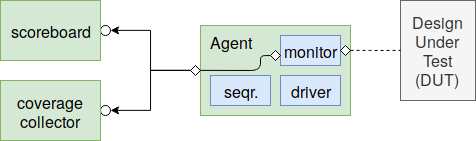
\includegraphics[width=100mm]{img/v8_analysis_components.png}
  \caption{Primer komponenti za analizu}
  \label{fig:analysis_components}
\end{figure}

Korišćenje TLM interfejsa je veoma često za analizu tj. u komponentama koje
služe za nadgledanje aktivnosti DUT-a i analizu prikupljenih podataka. Te
komponente su uglavnom monitori, \emph{scoreboard}-i, eventualni sakupljači
pokrivenosti, itd. Neke od ovih komponenti su prikazane na slici
\ref{fig:analysis_components}. Monitor će nadledati same signale preko
virtuelnog interfejsa i vršiće konverziju iz nivoa signala u nivo transackcija.
Te prikupljene transakcije će tada preko portova za analizu (\emph{analysis
  port}) slati ostalim komponentama na dalju obradu. U \emph{scoreboard}-u će se
prikupljati transackcije i vršiti provera da li DUT funkcioniše u skladu sa
funkcionalnom specifikacijom, \emph{coverage collector} će prikupljati podatke o
pokrivenosti, itd. Kako bi ovaj mehanizam ispravno funkcionisao potrebno je u
svakoj komponenti dobro definisati TLM interfejs i zatim izvršiti njihovo
povezivanje. Sledi opis ovog mehanizma.\\

Napomena: iako je moguće sve prethodne funkcionalnosti obaviti u jednoj
komponenti, dobra je praksa da se odvoji na više komponenti kako bi se omogućila
lakša ponovna upotreba i veća čitljivost koda.\\

Česta topologija koja se sreće u praksi je \emph{one-to-many} odnosno iz jednog
izvora se šalju podaci na više mesta (monitor ka \emph{scoreboard}-u,
\emph{coverage collector}-u itd), pri čemu ne postoji ograničenje za broj
primaoca. U UVM-u postoje tri objekta koji se mogu koristiti za ove svrhe:
\emph{analysis port}, \emph{analysis export} i \emph{analysis fifo}.\\

\emph{Analyisis port} se koristi kako bi se obavio neblokirajući
\emph{broadcast} transakcija. Za svaki port se može vezati više komponenti koje
će primati poruke, ali je moguće i da nijedna komponenta ne bude povezana.
\emph{uvm\(\_\)analysis\(\_\)port} sadrži jednu funkciju, \emph{write()}, čija
se implementacija nalazi u komponenti koja prima transakcije. Pozivom
odgovarajuće \emph{write()} funkcije se vrši slanje transakcija. U nastavku je
data sintaksa deklarisanja i primer korišćenja:

\begin{lstlisting}
class monitor extends uvm_monitor;

  uvm_analysis_port#(trans) ap;

  function new(string name = "monitor", uvm_component parent = null);
    super.new(name, parent);
    ap = new("ap", this);
  endfunction

  task main_phase(uvm_phase phase);
    trans t;
    // ...
    ap.write(t);
  endfunction

endclass
\end{lstlisting}

Sintaksa za deklarisanje analysis porta je: \emph{uvm\(\_\)analysis\(\_\)port
\(\#\)(\textless tip\textgreater ) \textless ime\textgreater ;} Zatim je
potrebno kreirati port u konstruktoru. Slanje podatka svim povezanim
interfejsima vrši se pozivom funkcije \emph{write} čiji je prototip:
\emph{function void write (input T t)}. Sama implementacija ove funkcije nalazi
se u komponenti koja treba da prima transakcije odnosno sadrži
\emph{uvm\(\_\)analysis\(\_\)imp}. Primer ovakve komponente je dat u nastavku:

\begin{lstlisting}
class scbd extends uvm_scoreboard;

  uvm_analysis_imp#(trans, scbd) ap;

  function new(string name = "scbd", uvm_component parent = null);
    super.new(name, parent);
    ap = new("ap", this);
  endfunction

  function void write(trans t);
    // ...
  endfunction

endclass
\end{lstlisting}

Svaki put kada se u \emph{mon} klasi želimo da pošaljemo transakciju \emph{sb}
komponenti pozove se funkcija \emph{write}. Međutim, postoje određena pravila
za implementaciju ove funkcije. Pošto je u pitanju funkcija, a ne task ne sme se
trošiti simulaciono vreme. Takođe, nije dozvoljeno modifikovanje prosleđene
vrednosti odnosno objekta \emph{t}.\\

Povezivanje \emph{uvm\(\_\)analysis\(\_\)port}-a i
\emph{uvm\(\_\)analysis\(\_\)imp}-a se uglavnom vrši u komponentama na višem
nivou hijerarhije. Na primer, u \emph{connect} fazi agenta ili okruženja. Kako
bi se izvršilo povezivanje, potrebno je pozvati metodu \emph{connect}, npr
(\emph{mon} i \emph{sb} su imena instanci):

\begin{lstlisting}
mon.ap.connect(sb.ap);
\end{lstlisting}

Pozivom ove funkcije smo povezali i drajver i sekvencer na prethodnim vežbama.
Ukoliko je potrebno povezati više koponenti na isti port, sintaksa ostaje ista,
pri čemu treba napomenuti da su sve komponente koje se povezuju na ovaj port
nezavisne odnosno svaka mora sadržati implementaciju svoje \emph{write}
funkcije. Npr.

\begin{lstlisting}
mon.ap.connect(sb1.ap);
mon.ap.connect(sb2.ap);
mon.ap.connect(sb3.ap);
\end{lstlisting}

Česta situacija je i da jedna komponenta treba da prima transakcije iz više
izvora. Npr. \emph{scoreboard} koji će primati transakcije iz više monitora u
okruženju i vršiti poređenje. U ovom slučaju je potrebno koristiti posebne
makroe za \emph{uvm\(\_\)analysis\(\_\)imp} kako bi se jasno definisalo koja
\emph{write} funkcija se odnosi na koji port.\\

U primeru ispod je data implementacija \emph{scoreboard} komponente koja sadrži
dva \emph{analysis\(\_\)imp}-a. Koristi
\emph{\`\ uvm\(\_\)analysis\(\_\)imp\(\_\)decl(\textless ime\textgreater )} makro
kako bi se deklarisala \emph{uvm\(\_\)analysis\(\_\)imp\textless
  ime\textgreater} klasa. Ovim se zatim kreira \emph{write\textless ime
  \textgreater ()} funkcija koju zatim možemo implementirati u skladu sa datim
potrebama.\\

Napomena: Imena korišćena u primeru (\emph{\(\_\)in} i \emph{\(\_\)out}) su
proizvoljna, ali je dobra praksa da započinju znakom ``\(\_\)'' pošto tada
rezultujuće \emph{write} funkcije imaju jasna imena (\emph{write\(\_\)in} i
\emph{write\(\_\)out}).

\begin{lstlisting}
`uvm_analysis_imp_decl(_in)
`uvm_analysis_imp_decl(_out)

class scbd extends uvm_scoreboard;

  uvm_analysis_imp_in#(trans, scbd) port_in;
  uvm_analysis_imp_out#(trans, scbd) port_out;

  function new(string name = "scbd", uvm_component parent = null);
    super.new(name, parent);
    port_in = new("port_in", this);
    port_out = new("port_out", this);
  endfunction

  function void write_in(trans t);
    // ...
  endfunction

  function void write_out(trans t);
    // ...
  endfunction

endclass
\end{lstlisting}

Povezivanje ove komponente bi se vršilo na isti način, tj:

\begin{lstlisting}
mon1.ap.connect(sb.port_in);
mon2.ap.connect(sb.port_out);
\end{lstlisting}

%========================================================================================
% Section
%========================================================================================

\section{Monitor}

Monitor komponenta je zadužena za izvlačenje informacija iz signala i
prevođenje u viši nivo apstrakcije bilo u vidu transakcija, događaja ili nekih
statusnih informacija. Ove informacije treba da su dostupne ostatku okruženja
preko TLM interfejsa. Monitor je uvek pasivna komponenta zadužena za nadgledanje
signala, a ne i njihovo generisanje. Iako se deo funkcionalnosti monitora često
preklapa sa funkcionalnošću drugih komponenti (uglavnom drajvera), monitor mora
biti nezavisna komponenta. Funkcionalnost monitora treba ograničiti na osnovno
nadgledanje koje će uvek biti potrebno, ali koje može biti i lako kontrolisano
npr. provere protokola ili sakupljanje pokrivenosti. Sve naprednije
funkcionalnosti (npr. provere vezane ne samo za protokol, već za naprednu
funkcionalnost DUT-a) treba implementirati u odvojenim komponentama -
\emph{scoreboard}-u, prikupljaču pokrivenosti, globalnim monitorima i sl.
Takođe se često odvaja i izvlačenje informacija iz signala od aktivnosti nad
transakcijama. Za sve komunikacije između pod-komponenti treba koristiti TLM
portove.

% ----------------------------------------------------------------------------------------

\subsection{Struktura}

U najosnovnijem obliku, monitor će sadržati virtualni interfejs preko koga
pristupa signalima, \emph{analysis port} za slanje prikupljenih transakcija i
\emph{factory} registraciju. Kostur UVM monitora je dat ispod. U \emph{connect}
fazi se vrši preuzimanje interfejsa in baze, dok se u \emph{run} ili \emph{main}
fazi vrši prikupljanje podataka i slanje preko TLM porta.

\lstinputlisting[caption=Kostur monitora, label=lst:calc_monitor]{code/v8_calc_monitor.sv}

Česta, ali ne i obavezna, praksa je da monitor sadrži kontrolna polja (u primeru
\emph{checks\(\_\)enable} i \emph{coverage\(\_\)enable}) koja služe za kontorlu
obavljanja čekiranja i prikupljanja pokrivenosti. Ove operacije mogu veoma
uticati na brzinu simulacije, pa je potrebno obezbediti način da se one, po
potrebi, isključe.

\begin{lstlisting}
if (checks_enable)
  perform_transfer_checks();
if (coverage_enable)
  perform_transfer_coverage();
\end{lstlisting}

Kontrolu je tada lako vršiti koristeći mehanizam konfiguracija, npr:

\begin{lstlisting}
uvm_config_db#(int)::set(this,"*.monitor", "checks_enable", 0);
\end{lstlisting}

% ----------------------------------------------------------------------------------------

\subsection{Funkcionalnost}

Glavna razlika između drajvera i monitora je što je monitor pasivna komponenta.
Ovo znači da je monitor zadužen samo za nadgledanje signala, a ne i njihovo
generisanje. Kako bi ispravno prepoznao aktivnosti na signalima, monitor mora
poznavati protokol koji se koristi. Praćenje određenog protokola se često
implementira kao mašina stanja u \emph{run/main} fazi.
Čeka se na određene događaje odnosno prate se stanja signala preko virtuelnog
interfejsa.
Nakon što se uoči šablon datog protokola, potrebno je kreirati objekat koji
predstavlja transakciju i dodeliti mu odgovarajuće vrednosti (npr. trenutna
operacija, adresa, vrednost podataka, ...).
Nakon što se objekat uspešno kreira, šalje se svim ostalim komponentama pomoću
TLM interfejsa.
Nadgledanje signala se obično vrši u beskonačnoj petlji u \emph{run/main} fazi.
Prilikom svakog prolaska kroz petlju, šalje se uočena transakcija.
Pošto objektu pristupamo preko pokazivača, problem koji se može javiti je da se
vrednosti prebrišu u narednoj iteraciji.
Ovo je moguće izbeći na dva načina:

\begin{itemize}
\item Kreiranje novog objekta u svakoj iteraciji petlje
\item Koristiti isti objekat, ali izvršiti kloniranje pre poziva \emph{write} funkcije i poslati klon
\end{itemize}

U nastavku je dat primer \emph{main} faze APB monitora:

\lstinputlisting[caption=Main faza APB monitora, label=lst:apb_main_phase]{code/v8_apb_main_phase.sv}

% ----------------------------------------------------------------------------------------

\subsection{Implementacija čekera}

Dve glavne funkcionalnosti monitora, pored sakupljanja transakcija, su vršenje
provera i prikupljanje podataka o pokrivenosti. Prikupljanju pokrivenosti
(\emph{coverage}) će biti posvećena posebna vežba, dok ćemo se u ovoj vežbi
zadržati na preporučenom načinu implementacije čekera.

\subsubsection{\emph{Assert} naredbe}

\emph{Assert} naredbe se primarno koriste za proveru funkcionalnosti dizajna,
ali i za proveru samog verifikacionog okruženja (npr. provera uspešnosti
randomizacije). U SystemVerilog-u postoje dve vrste ovih tvrdnji:

\begin{itemize}
\item trenutne (\emph{immediate}): proceduralne naredbe koje se uglavnom koriste
  tokom simulacije; tvrdnja koja govori da neki izraz mora biti tačan, nalik if
  naredbi; veoma liče na \emph{assert} naredbe u VHDL-u
\item konkurentne (\emph{concurrent}): naredbe koje govore da neke osobine
  dizajna moraju biti ispunjene (npr. \emph{read} i \emph{write} signali ne
  smeju biti aktivni u isto vreme ili posle svakog \emph{request}-a sledi
  \emph{acknowledge}).
\end{itemize}

Pisanje \emph{concurrent assertion}-a izlazi iz opsega ovog kursa, međutim za
implementaciju čekera je preporučeno koristiti \emph{immediate assertion}, što
je opisano u nastavku.\\

U monitoru, čekere je moguće pisati koristeći običan proceduralni kod ili
trenutne tvrdnje. U primerima ispod proverava se da li je vrednost A jednaka
vrednosti B. Razlika je sledeća: korišćenjem if naredbe se samo proverava da li
je A == B, a sve dalje akcije je potrebno posebno definisati, dok druga naredba
tvrdi da je A == B i vratiće grešku ukoliko ovo nije ispunjeno.

\begin{lstlisting}
if (A == B) // ...
assert (A == B);
\end{lstlisting}

Prednosti korišćenja tvrdnji su mnogobrojne. Ovim naredbama se povećava
čitljivost koda, ali i smanjuje vreme potrebno za \emph{debug} jer je greške
lakše izolovati i brže uočiti. Simulatori pružaju mogućnosti nadgledanja broja
tvrdnji koje prolaze ili ne, pauziranje simulacije ukoliko se pronađe greška,
... Takođe pružaju veliku mogućnost kontrole tokom samog testa npr. moguće je
uključiti ili isključiti ove provere. Moguća je i interakcija sa C funkcijama.
Prednosti se takođe ogledaju u pogledu dokumentacije jer olakšavaju opis čekera
i dizajn specifikacije.\\

Sintaksa immediate tvrdnje je sledeća:

\begin{lstlisting}
assertion_label : assert (expression)
  // pass block code
else
  // fail block code
\end{lstlisting}

gde je labela opciona, kao i \emph{pass} i \emph{fail} blokovi koda. Dobra
praksa je da se u \emph{fail} bloku ispiše poruka koja objašnjava zašto je došlo
do greške. Takođe je korisno da se koristi labela kako bi se lakše pratile sve
tvrdnje u okruženju (često ima prefiks ili sufiks \emph{asrt}). Primer je dat
ispod:

\begin{lstlisting}
asrt_a_eq_b : assert (A == B)
  `uvm_info(get_type_name(), "Check succesfull: A == B", UVM_HIGH)
else
  `uvm_error(get_type_name(), $sformatf("Observed A and B mismatch: A = %0d, B = %0d", A, B))
\end{lstlisting}
% $

%========================================================================================
% Section
%========================================================================================

\section{Zadaci}

\paragraph{Zadatak}

Implementirati monitor za ``Calc1'' dizajn.

%========================================================================================
% Section
%========================================================================================

\section{Appendix}

\lstinputlisting[caption=calc\(\_\)if, label=lst:calc_if]{code/calc_if.sv}
\lstinputlisting[caption=v8\(\_\)calc\(\_\)sequencer, label=lst:v8_sequencer]{code/v8_calc_sequencer.sv}
\lstinputlisting[caption=v8\(\_\)calc\(\_\)driver, label=lst:v8_driver]{code/v8_calc_driver.sv}
\lstinputlisting[caption=v8\(\_\)calc\(\_\)monitor, label=lst:v8_calc_monitor]{code/v8_calc_monitor.sv}
\lstinputlisting[caption=v8\(\_\)calc\(\_\)seq\(\_\)item, label=lst:v8_seq_item]{code/v8_calc_seq_item.sv}
\lstinputlisting[caption=v8\(\_\)calc\(\_\)agent\(\_\)pkg, label=lst:v8_calc_agent_pkg]{code/v8_calc_agent_pkg.sv}
\lstinputlisting[caption=v8\(\_\)test\(\_\)base, label=lst:v8_test_base]{code/tests/v8_test_base.sv}
\lstinputlisting[caption=v8\(\_\)test\(\_\)simple, label=lst:v8_test_simple]{code/tests/v8_test_simple.sv}
\lstinputlisting[caption=v8\(\_\)test\(\_\)simple\(\_\)2, label=lst:v8_test_simple_2]{code/tests/v8_test_simple_2.sv}
\lstinputlisting[caption=v8\(\_\)calc\(\_\)test\(\_\)pkg, label=lst:v8_calc_test_pkg]{code/tests/v8_calc_test_pkg.sv}
\lstinputlisting[caption=v8\(\_\)calc\(\_\)base\(\_\)seq, label=lst:v8_calc_base_seq]{code/sequences/v8_calc_base_seq.sv}
\lstinputlisting[caption=v8\(\_\)calc\(\_\)simple\(\_\)seq, label=lst:v8_calc_simple_seq]{code/sequences/v8_calc_simple_seq.sv}
\lstinputlisting[caption=v8\(\_\)calc\(\_\)seq\(\_\)pkg, label=lst:v8_calc_seq_pkg]{code/sequences/v8_calc_seq_pkg.sv}
\lstinputlisting[caption=v8\(\_\)calc\(\_\)verif\(\_\)top, label=lst:v8_calc_verif_top]{code/v8_calc_verif_top.sv}
%========================================================================================
